\chapter{Sorting and searching algorithms}

\begin{goals}
\item Understand why designing efficient algorithms is important and how to measure algorithms' performance
\item Understand why sorting and searching algorithms are important
\item Understand the basic sorting/searching methods
\item Learn how to implement these methods
\end{goals}

 \section{Algorithm analysis}
 
 We will start off this chapter by building an intuitive understanding of why different implementations of the same algorithm have different performance (running time). We will first discuss how to observe and model performance characteristics of algorithms and then discuss how we can classify the algorithms based on the order of growth of their running time. 

Understanding how to compare the performance of different algorithms and provide guarantees on how well they perform will help us learn and compare the sorting and searching algorithms we will be considering later in this chapter. 


The main reason we would like to have a sense of the performance of an algorithm is to be able to tell whether the program can solve a large practical input or not. Given two computer programs that perform the same task, how can we tell which program is 'faster'? The most straightforward way is to time each program, for example, using the stopwatch. However, here, we assume that the two programs are run on the same computer to make the comparison fair. We can not make a meaningful comparison of the two programs if we ran them on different computers because even running the same programs on two different computers would likely lead to two different running times since one computer might have a better hardware (processor speed, memory, disk space). 

Therefore, this way of measuring the performance of an algorithm is not the most convenient one. Another way of measuring the performance independent of the type of computer we use is by counting the number of instructions or operations in the two programs. Usually, the faster program has fewer operations. Intuitively, we would also expect that the number of operations is proportional to the number of data items that the program operates on. 



Donald Knuth pioneered the following approach to understating the total running time of a program:

Total running time: sum of cost $\times$ frequency of all operations.

Therefore, we need to analyze a program to determine the set of operations it uses. The cost depends on the machine and the compiler. The frequency of the operations depends on the algorithm as well as input data. 

\begin{exercise}
\begin{code}
int count = 0;
for (int i = 0; i < N; i++)
	If (a[i] == 0)
		count++;
\end{code}

For each operation (variable declaration, assignment statement, less than compare, equal compare, array access, increment), determine its frequency of execution as a function of input size $N$.

\end{exercise}



Though, in theory, we could determine the running time of a program using Donald Knuth’s method, we usually don’t need to know the running time with such precision. We can approximate the running time by making the following simplifications: 1) use some basic operation (perhaps the one that costs the most) as a proxy for running time; 2) only consider the highest order terms in our derivation of the running time. For example, if we derived the running time to be $\frac{1}{2}N^3 + 50 N$, we would approximate this with ~ $\frac{1}{2}N^3$.

Next, it turns out that the following set of functions 
$1, logN, N, NlogN, N^2, N^3, 2^N$
suffices to describe order-of-growth of typical algorithms. 


\section{Sorting and searching algorithms}

How do you find a friend's phone number in the phone book? If a deck of cards has less than 36 cards, how do you determine which card is not in the deck?

As you can see, searching and sorting items are tasks you are familiar with from everyday life. Searching and sorting are also important in programming. For example, in your Word document, you can search for all occurrences of a word in the text in order to replace it with another word. You can sort files on your computer into alphabetical or numerical order based on the first character of the file's name. Thus, because searching and sorting are common and important computer tasks, programmers in the past have spent a lot of time developing sorting and searching algorithms. However, as you will see later, developing a sorting or searching algorithm is not enough: you need to design it to run as fast as possible so that it can be executed in a reasonable amount of time when we supply it with millions or billions of items to sort or search.


 
 Formally, the sorting problem is to rearrange items in an array into ascending order. For example, you would use a sorting algorithm if you wanted to display your email messages in reverse order of the time you received them. Generally, sorting is useful because it makes searching for an item in an array much easier. Both sorting and searching are important tools in commercial and scientific applications (e.g. keep record of your customers, organize your experimental data, etc.).

In general, when writing a program, we’d like to quantify the correspondence between the problem size and running time. Such analysis allows us to estimate how efficient a particular algorithm is. Moreover, it turns out that we can classify algorithms according to their performance as the problem size grows.

Many different implementations of sorting and searching algorithms have been proposed. When choosing a specific implementation, we should pay attention to the efficiency of a given algorithm and its performance characteristics. 

In this chapter, we will consider basic algorithms for searching (binary search) and sorting (insertion sort mergesort, quicksort).  



\section{Binary search}

Suppose you need to guess the value of a secret number which is an integer between 0 and $n-1$. When you make a guess $x$, you ask whether the secret number is greater than or equal to $x$ and receive \textit{true} or \textit{false} as an answer. For now, we will assume that $n$ is a power of 2.

The most straightforward approach is the following: since in each step, we ask a question (“is the number greater than or equal to $x$?”) that allows us to shrink the searching interval by half. In particular, we guess the number in the middle of the interval, and, based on the answer, discard the half of the interval that can not contain the secret number. For example, suppose we have a secret number 5 that is contained in an array of integers from 0 to 16. You guess $x=8$ (i.e. the middle of the array) and ask if the secret number is greater than or equal to $x$. You receive \textit{false} answer (since $5 < 8$); therefore, you can shrink the array to $[a;b) = [0, 8)$ and search for the secret number in this new array since you know for sure that the secret number is less than 8. Note that we denote the start of the new array of integers by $a$ and the end by $b$.  
We can summarize this approach in the following recursive strategy:

\begin{itemize}
\item \textit{Base case:} if $a-b = 1$, then the secret number is $a$.
\item \textit{Reduction step:} If not, ask whether the secret number is greater than or equal to the number $middle = a + (a+b)/2$. If the answer is \textit{true}, look for the number in  $[middle; b]$. If the answer is \textit{false}, look for the number in $[a; middle]$.
\end{itemize}

This searching strategy is called \textit{binary search}. Figure \ref{fig:binary} shows another example of how you would find number 23 in a given array using the binary search algorithm.

\begin{figure}
    \centering
    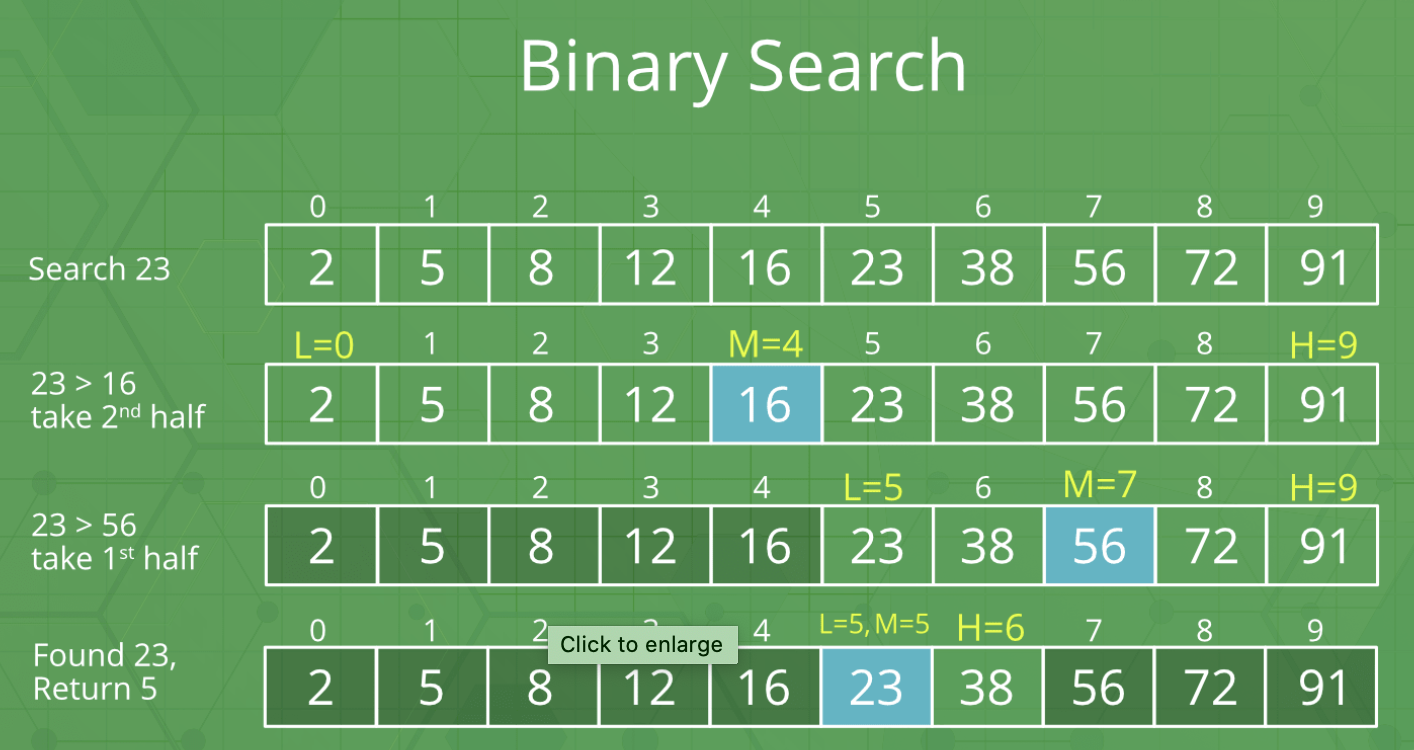
\includegraphics[width=\textwidth]{images/binary.png}
    \caption{An example of using binary search to find number 23 in the given array. \href{https://www.geeksforgeeks.org/binary-search/}{\textit{Source}}}
    \label{fig:binary}
\end{figure}


Below is an example implementation of binary search in Java.

\begin{code}
public class Example
{
    public static int binarySearch(int a, int b)
	{
	if (a-b == 1) return a;
 	int middle = a + (a-b)/2;
	StdOut.print("Is the secret number greater than or equal to " + middle + "? ");
	if (StdIn.readBoolean())
		return binarySearch(middle, b);
	else
		return binarySearch(a; middle);
	}
	public static void main(String[] args)
{
int k = Integer.parseInt(args[0]);
int n = (int) Math.pow(2, k);
StdOut.println("Choose a secret number between 0 and " + (n-1));
int guess = binarySearch(0, n)
StdOut.println("The secret number is " + guess);
}
}
\end{code}
 
 
 Mathematically, we can show that $T(n) = lg n$ where $T(n)$ is the number of questions. This, the running time of binary search is logarithmic.

\subsection{Binary search in a sorted array}
An important application of binary search is when we would like to find a piece of information using a key to guide the search. For example, in the last century people would use a phone book to look up a person’s phone number. In this case, the elements are sorted by a key (i.e. a person’s name, sorted in alphabetical order). Nowadays, we can implement this searching process using binary search.



\section{Insertion sort}

Now, we would like to discuss a few of the most fundamental sorting algorithms. 
Let’s start with a brute force algorithm known as \textit{insertion sort}. This algorithm mimics a method that people usually use to arrange hands of playing cards. Consider the cards one at a time and insert each into its proper place among those that have already been considered. Below is an example Java method that rearranges the strings in an array to put them in ascending order:

\begin{code}
public static void sort(String[] a)
{
	int n = a.length;
	for (int i = 1; i < n; i++)
		for (int j = i; j > 0; j- -)
			if (a[j-1].compareTo(a[j]) > 0)
				exchange(a, j-1, j)
			else break;

}
 
\end{code}
 
 
 At i-th iteration of the outer \textit{for} loop, the first I elements in the array are in sorted order; the inner \textit{for} loop moves a[i] into its proper position in the array. Note that the running time of insertion sort is sensitive to its input values. For example, if the input array happened to be already sorted, the running time of the program is linear. However, if the input array is in reversed order, then the running time is quadratic. There are many real-world applications for which insertion sort is quadratic, so we need to consider faster sorting algorithms.

\begin{figure}
    \centering
    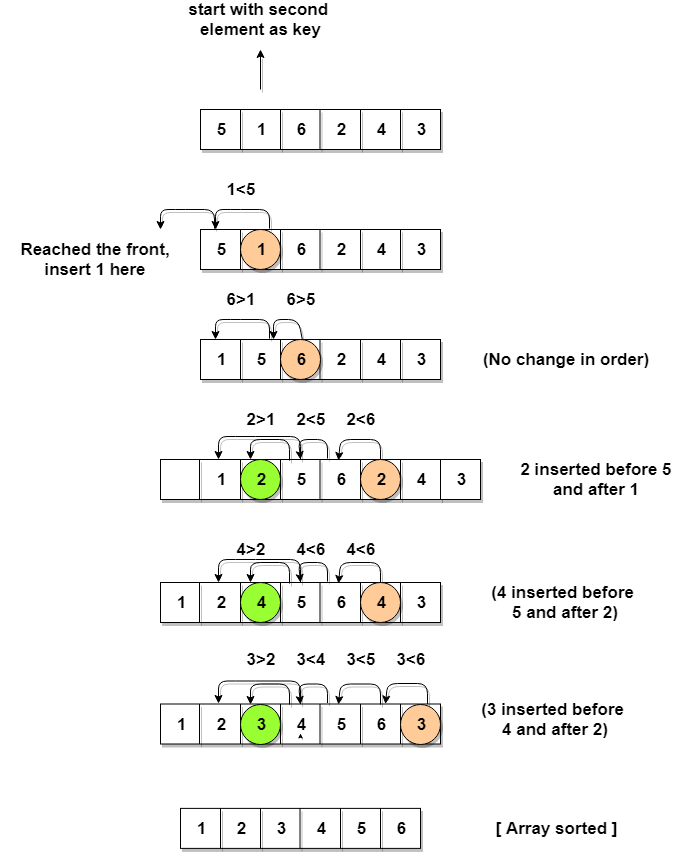
\includegraphics[width=\textwidth]{images/insertion-sort.png}
    \caption{An example showing how the insertion sort algorithm works. \href{https://vivaharsha.com/product/verilog-implementation-of-insertion-sort-16-bits-and-5-inputs/}{\textit{Source}}}
    \label{fig:insertion_sort}
\end{figure}


\section{Mergesort}
To create a faster sorting method, we need to understand recursion and a \textit{divide-and-conquer} approach to algorithm design. \textit{Divide-and-conquer} approach refers to the idea that we can solve a problem by \textit{diving} it into in depend parts, \textit{conquer} them independently, and then use the solution for the parts to develop a solution to the original problem. Applying this approach to sorting, we can first divide an array into two halves, sort the two halves independently, and then \textit{merge} the results into the full array. This sorting algorithm is called \textit{mergesort}. 

We consider contiguous subarrays of a given array \textit{array}, using the notation [a;b) to refer to the array consisting of elements array[a], array[a+1], …, array[b-1]. The mergesort algorithm implements the following strategy:
   
\begin{itemize}
\item \textit{Base case:} if the subarray length is 0 or 1, it is already sorted.
\item \textit{Reduction step:} If not, compute $middle = a + (a+b)/2$, recursively sort the two subarrays array[a, middle) and array[middle, b] and merge them.
\end{itemize}

You can view a short video that shows an example of how the mergesort algorithm works \href{https://youtu.be/4VqmGXwpLqc}{\textit{here}}.




\begin{exercise}

Fill in the blanks in the implementation of the mergesort algorithm.
\begin{code}

public void merge(int[] list, int low, int high) {
// temporary array stores the "merge" array within the method.

int[] temp = new int[list.length];
    // Set the midpoint and the end points for each of the subarrays
    int mid = (low + high)/2;
    int index1 = 0;
    int index2 = BLANK ;
    int index3 = mid + 1;
    // Go through the two subarrays and compare, item by item,
    // placing the items in the proper order in the new array
    while (index2 <= mid && index3 <= high) {
        if (list[index2] < list[index3]) {
            temp[index1] = list[index2];
            index1++;
            index2++;
}
else {
            temp[index1] = BLANK;
            index1++;
            index3++;
} }
    // if there are any items left over in the first subarray, add them to
    // the new array
    while (index2 <= mid) {
        temp[index1] = list[index2];
        index1++;
        index2++;
}
    // if there are any items left over in the second subarray, add them
    // to the new array
    while (index3 <= high) {
        temp[index1] = list[index3];
        index1++;
        index3++;
}
    // load temp array's contents back into original array
    for (int i=low, j=0; i<=high; i++, j++) {
        list[i] = BLANK;
    }
}

 
\end{code}
 

\end{exercise}
 
 Mathematically, we can show that the running time of mergesort is linearithmic.
 
 
 \section{Quicksort}
 
 
 Another sorting divide-and-conquer algorithm is called \textit{quicksort}. It works by \textit{partitioning} an array into two parts and then sorting the parts independently. The main feature of this sorting algorithm is the partiotioning process, which rearranges the array to make three conditions hold:

\begin{itemize}
\item The entry array[j] is in its final place in the array, for some j
\item No entry in array[a] through array[j-1] is greater than array[j]
\item No entry in array[j+1] through array[b] is less than array[j]
\end{itemize}

With this algorithm, we do the sorting by first partitioning the array and then applying this method recursively to the subarrays of the array. This algorithm shuffles the array before sorting it. 

\textbf{Partitioning} To implement the quicksort algorithm, we first need to implement the partitioning method. First, we arbitrarily choose array[a] to be the partitioning item, which will go into its final position. Next, we search from the left end of the array for an entry that is greater than or equal to the partitioning item. We then search from the right end of the array for an entry that is less than or equal to the partitioning item.The two found items are out of place so we exchange them. When the scan indices cross, to finish the partitioning process we need to exchange the partition item array[a] with the rightmost entry of the left subarray (array[j]) and return its index j.



You can view a short video that shows an example of how the quicksort algorithm works \href{https://youtu.be/Hoixgm4-P4M}{\textit{here}}.

\begin{figure}
    \centering
    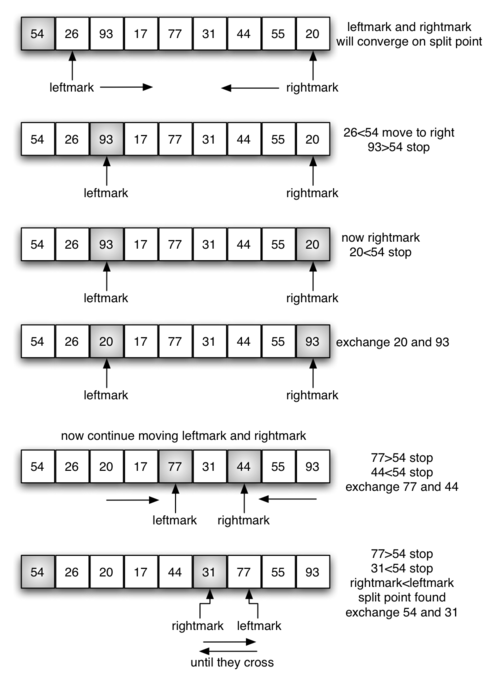
\includegraphics[width=\textwidth]{images/quicksort.png}
    \caption{An example showing how the quicksort algorithm works. \href{https://runestone.academy/runestone/books/published/pythonds/SortSearch/TheQuickSort.html}{\textit{Source}}}
    \label{fig:insertion_sort}
\end{figure}


\begin{exercise}
Choose your favorite searching or sorting algorithm and run experiments with different input sizes to determine how the running time of the program changes with the input size. Run the algorithms on ten different input sizes and make a plot of the running time as a function of the input size.

\end{exercise}